
\documentclass[english]{tktltiki}
\usepackage[pdftex]{graphicx}
\usepackage{graphicx}
\usepackage{subfigure}
\usepackage{url}
\usepackage{xcolor}
\usepackage{amsmath}
\begin{document}


\onehalfspacing
\title{Reinforcement Learning in Games: A Mini Survey}
\author{Ege Can �zer}
\date{\today}

\maketitle
\numberofpagesinformation{\numberofpages\ pages + \numberofappendixpages\ appendices}

\classification{\protect{\ \\
	A.1 [Introductory and Survey],\\
	I.7.m [Document and text processing]}}

\keywords{Reinforcement learning, Convergence and learning in games}

\begin{abstract}
    Self-learning programs have been studied and applied in many different fields; but recently, it gains more popularity and familiarity due to its breakthrough success in the gaming domain. Unlike the examples are taken from the real world, having the predefined set of rules and the less complicated environment in this domain provides greater flexibility to develop reinforcement learning algorithms. However, there are also several difficulties to resolve to be able to study reinforcement learning in games. We will identify these challenges and present an example approach.
    
    In this paper, we will study the applications of reinforcement learning algorithms in the gaming context by closely focusing on four different articles. Based on the findings, we hope to propose possible improvements for future studies.
\end{abstract}

\mytableofcontents

\section{Introduction}
During the last decade, reinforcement learning paradigm has gained a decent amount of popularity. Since middle 80's it has been applied in many fields to address complex problems such as in robotics, control systems, finance, and agent-based systems due to its generic formulation. In its essence, reinforcement learning looks for optimal input actions that maximize the output states by making use of the feedbacks from the environment \cite{sutton1998introduction}. In spite of the fact that reinforcement learning being a mature and widely-used concept, the primary reason to get such attention recently is due to breakthrough success in the gaming context \cite{mnih2013playing, silver2016mastering}.

Studying reinforcement learning algorithms in the gaming context contributes several definitive advantages \cite{tesauro1995temporal}. In general, modeling of the problem, implementation, and analysis of the results in real life examples are harder than the artificial ones such as games. Moreover, having simplified and controlled environment, as well as specifically defined rule sets not only allow an opportunity to explore the new variety of reinforcement learning algorithms, but also enable to have concrete evaluation measurements. Further, research results are reproducible, easy to simulate and provide test-bed for future studies. Therefore, for the given reasons, studying reinforcement learning in games can help the field to progress further and more effectively.

On the other hand, there are many difficulties to resolve to be able to study reinforcement learning algorithms in games. Implementation perspective being one of them that reinforcement learning algorithms require a proper playground for simulations. The performance measure is also another challenge in this domain, mainly because hand-labeled ground truth sets are not relevant in reinforcement learning, unlike in supervised learning. Further, deciding how to handle the complex game environment is a demanding task. Since the agent's performance and features are highly correlated, results may lead to extremely slow convergence or not at all. Given these points, we undertake to inspect the challenges of reinforcement learning algorithms in games.

In this article, we examine four existing reinforcement learning systems in the gaming domain. First, Liao et al. \cite{liao2012cs229} introduce a single learner to play classic platformer game, using $\varepsilon$\textit{-greedy} Q-learning. Second, Amato and Shani \cite{amato2010high} demonstrate high-level reinforcement learning approach to improve the built-in AI of a turn-based strategy game. Third, Gerald Tesauro \cite{tesauro1995temporal} proposes a first successful combination of reinforcement learning and neural network system that achieves human grandmaster level. Finally, Mnih et al. \cite{mnih2013playing} demonstrate a deep reinforcement learning model that learns control policies directly from sensory input and accomplishes remarkable results.

The rest of this paper is organized as follows. In section 2, we discuss common challenges and approaches to the problems in reinforcement learning in games such as dealing with the abstraction of the environment or evaluation of the results. In section 3, we review existing systems in detail each with its unique characteristics and give a comparative analysis. The last section summarizes and concludes the paper.

\section{Challenges and  approaches}
In the last decade, many research has gone into investigating reinforcement learning algorithms in games. Concurrently, many challenges and approaches have arisen around this topic repeatedly. In this section, we present some of those common challenges and some approaches that exist mostly in the reviewed systems \cite{tesauro1995temporal, amato2010high, liao2012cs229, mnih2013playing}.

Because there exist many different and specific problems as well as methods to tackle them, the challenges and approaches listed in this section are all related but not necessarily belong to every system in the whole research field. Generally, given matters are all common, but still, some of them may not appear within another context.

\subsection{Implementation perspective}
Reinforcement learning researchers require robust playground to train and test the system. Nonetheless, finding the platform, considering the medium, and how to evaluate results has to be chosen in a manner that it does not misdirect the research. Because of the lack of freedom in the software, it can limit the research in a certain way. For example, researchers may end up building the whole playground from scratch. Therefore, finding appropriate software development kits are crucial even before considering the study reinforcement learning algorithms in this domain.

Fortunately, there exists plenty of variety in implementation, ranging from turn-based board games to fast-paced action games. It is not possible to have every specific game mainly due to the trademarking concerns, but some still open source the content or provide a refined framework for everyone. For example, we observe \cite{amato2010high, liao2012cs229, mnih2013playing} take advantage of different frameworks to train and as well as to test their system. So that using a common framework provides a reproducible and objective result. In all, having a proper playground to study reinforcement learning in the gaming context is unignorable and certainly an important aspect.

\subsection{Abstracting the environment}
In order to study the games properly using reinforcement learning, the very first step is abstracting the game environment in terms of Markov decision processes. This is because the modeling choices, as well as the definitions,  may differ based on the systems (for example, transition probability parameter does not exist in Q-learning). We are not going to give in-depth algorithmic analysis for any of the inspected systems in this paper. Therefore, we will follow one example model by Liao et al. \cite{liao2012cs229} to only illustrate the concept.

\begin{align}
Q(s_t, a_t) \leftarrow 
(1 - a_{s,a}) Q(s_t, a_t) + 
\alpha_{s,a}(r + \gamma max(Q(s_{t+1}, a_{t+1}))) \label{eq:mario}
\end{align}

We can inspect the required elements for a model more easily directly from the equation \ref{eq:mario}. In total \textit{five} factors need to be defined in this model. These are $ s_t $, the state space that the agent might be in, $ a_t $, the set of actions that agent capable of taking, $ r $, the reward function that the agent receives after transitioning from $s_t$ to $s_{t+1}$ via $ a_t $. The $\gamma \in [0,1]$ is the discount factor that serves as a tuning parameter for present and future rewards. Finally $ \alpha_{s,a} \in [0,1]$ is the learning rate that affects agent's convergence rate. Further details are stated in \cite{liao2012cs229}.

Liao et al. \cite{liao2012cs229} make use of the Mario AI framework to encode the game environment in the following way. From the figure \ref{fig:mario} it can be inferred that nearly any condition of the character and its surroundings can be extracted. According to the article, $s_t$ designed in a way that it requires 39 bits to encode in a state vector, such example attributes are Mario's current mode (small, big, fire), movement states, enemy distance within 3 different ranges and so on. There are 12 different $a_t$ that Mario agent can perform, from the combinations of (LEFT, RIGHT, STAY) x (JUMPY, NOT\_JUMP) x (SPEED/FIRE, NO\_SPEED). In the article, $r$ is defined as the combination of weighted state attribute values and the distance that agent performs from the last frame. $a_{s,a}$ and $\gamma$ parameters chosen based on several try-outs that would lead to a non-degenerated performance in the evaluation.

Overall, we revealed an example approach to encode a game environment to be able to make use of a reinforcement learning algorithm. Moreover, there are many ways to handle the abstraction of the game environment and making use of the reinforcement learning algorithms. However, we briefly categorize them in 3 possible ways, low-level, high-level and context-free abstraction based on the systems we reviewed. We refer the presented approach as the low-level abstraction, where the designer can access to nearly all attributes available from the environment and the agent explores all possibilities in the search space. If one can access only the limited resources and be able to utilize inner mechanics of the system, we refer to it as high-level modeling. Compare to previous one, this abstraction approach does not have huge search space. The last one, context-free modeling encodes the environment without any context related knowledge. In the literature, we observed that such modeling can be achieved by using convolutional neural networks \cite{mnih2013playing, silver2016mastering}. We will go over these abstraction methods as we examine systems in the further sections.

\begin{figure}[h]
	\begin{center}
		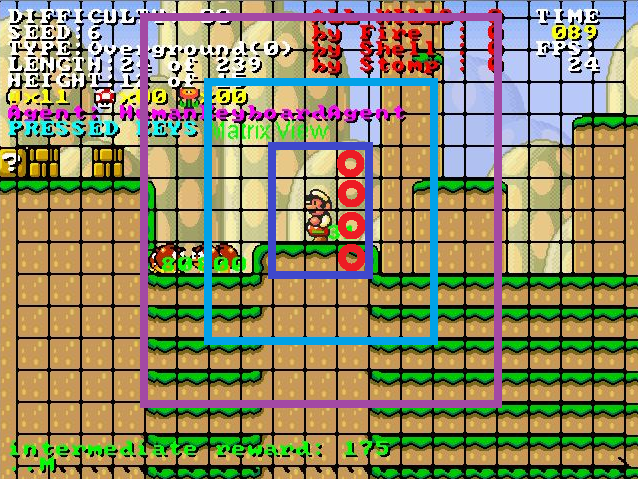
\includegraphics[width=0.65\textwidth]{img/mario.png}
		\caption{ Mario AI framework interface provides control over several variables. In the figure, 3 level distance to nearby enemies can be seen from the square fields around the main character. Liao et al. make use of this AI framework to implement their algorithm \cite{liao2012cs229}. }
		\label{fig:mario}
	\end{center}
\end{figure}



\subsection{Performance measures}
In reinforcement learning, it is crucial to assess the effectiveness of the algorithm, but because of the nature of "learning by experience" evaluation can be challenging. Unlike in supervised learning methods, which there is a ground truth dataset to evaluate the model, reinforcement learning methods would require millions of entries to be effective. Mainly because it takes many iterations to have an intermediate to expert level of an agent, and trying to use the same procedure for reinforcement learning would be a trivial and laborious task for researchers. Thus, one needs to consider other means of evaluation methods.

There are several different methods available to assess the quality of the model; however, we consider the groups that Gerald Tesauro \cite{tesauro1995temporal} states. According to this, we mention there are three different methods to evaluate reinforcement learning model. It is high-level, general enough to cover most of the systems, and actually used without a naming convention by others. Also for this paper, we will refer these groups in our comparative analysis later on.

The first method is evaluating the system using an automated benchmarking system. This can be seen as a computer opponent or an objective platform for all other AIs. One obvious advantage of using an automated tool is that the programs can be iterated over many times and accurate statistics can be obtained to support sufficient benchmarks.

The second method is evaluating the system against the master level human players. The major benefit of this method is that it can serve as a clue about the reference point of a play performed by the system. However, as the level of complexity increases in the games, the human knowledge may be erroneous and thus unreliable to serve as a ground truth. This seems to happen frequently in the history especially in the board games such as \cite{tesauro1995temporal, silver2016mastering}. Besides, the number of game plays against humans are more restricted and slower, specifically compared to previous one. But, the evaluation method still can aid for the given reason.

Last evaluation method is done by analyzing individual decisions by a system, which is actually closely related to the second method. It is valid to say that it also inherits nearly the same problems. Gerald Tesauro \cite{tesauro1995temporal} states that the method used to analyze the individual decisions via computer roll-outs in a backgammon game. However, one can induce this approach for any systems. The key thing is to set up candidate positions, just as in the supervised learning, and letting the computer to play out the position several times. The results can be deductible from the statistics of good and bad plays. However, it is more suitable for stochastic environments or having large state spaces, generally board games. 

\subsection{Further challenges}
Until now we bring up common problems that every reinforcement learning systems strive. Still, underlying all possible challenges, especially after the combinations of other fields, not only out of the scope of this paper but also an intractable and demanding task. For this reason, we will additionally cover only a few prominent ones from what we have studied. Briefly, these are exploration versus exploitation trade-off and various reinforcement learning challenges from deep learning point of view.

To begin with, exploitation versus exploration dilemma is truly one of the classic challenges in reinforcement learning. The problem comes along with the agent's main learning objective. That is, the agent must be able to obtain the maximum possible reward from the set of actions that it has performed before. But, it must discover such new actions that would also lead to maximizing the reward in future \cite{sutton1998introduction}. The dilemma is basically deciding on what is the perfect moment to explore and exploit, yet it has no single solution. Sutton and Barto \cite{sutton1998introduction} demonstrate ways to balance between exploration and exploitation, including $\varepsilon$\textit{-greedy} and \textit{softmax} which all are perform near-optimally reward. Even though there exist many possible techniques in the literature, upon closer examination $\varepsilon$\textit{-greedy} appears to be a common approach, also in \cite{amato2010high, liao2012cs229}.


On the other hand, reinforcement learning suffers many problems from deep learning point of view which some are identified by Mnih et al. \cite{mnih2013playing}. First, data needs to be independent and identically distributed based on the assumptions of deep learning algorithms. In contrast to this, reinforcement learning usually consists of sequences of highly correlated actions. Moreover, the vast majority of deep learning algorithms requires an extensive amount of labeled data to achieve "automatic" feature extraction, whereas reinforcement learning algorithms' experience-based learning demands reward that is usually noisy and delayed. Also, agents in reinforcement learning algorithms likely to change their behaviors as they explore, this indefinite data distribution violates the fixed distribution assumption of the deep learning algorithms. Fortunately, there exists deep learning approach to overcome these issues \cite{mnih2013playing}.

\section{Review of existing systems}

Until now we have seen that there are several challenges and approaches for the reinforcement learning algorithms. In order to get more intuition behind the matter, we have examined four unique systems. We demonstrate their adaptation to the challenges, and how they handle and make use of reinforcement learning in games. At the end of the section, we present a comparative analysis of reviewed articles.

\paragraph{Reinforcement Learning to Play Mario \cite{liao2012cs229}.}
The first article authored by Liao et al. \cite{liao2012cs229} focuses on the design of a single agent, which plays a classic platformer game called Super Mario Bros using, $\varepsilon$\textit{-greedy} Q-learning. The aim of the agent is to get the highest score. To acquire that it has to overcome various obstacles and gain rewards, such as beating enemies, avoiding gaps, or collecting items, until it reaches the finish line.

The authors used a framework called, Mario AI which helps to abstract the game environment at low-level, meaning many attributes tailored to encode into one state. The main motivation to use the $\varepsilon$\textit{-greedy} Q-learning algorithm is because the state transition probabilities do not need to be known by the algorithm beforehand. Moreover, the method ensures larger state space and faster computation time. $\varepsilon$\textit{-greedy} action selection extension provides a balanced way to explore more states, as well as decaying learning rate ensures faster converge policy rate than fixed learning rate. 

Using the same framework, training and evaluation of the agent are done under different learning parameters. The optimum one is selected based on the four performance metrics. After 5000 training iterations, the agent is able to reach approximately 90\% of winning probability ($\approx$ 9000 average score) of the game. On the other hand, evaluation of the system is only compared against baseline. Even though the tool by Karakovskiy and Togelius \cite{karakovskiy2012mario} provides several benchmarking tracks, none of the performance metrics present an objective comparison to existing systems. To be able to present definitive results, a possible benchmark or a human-level comparison could be applied. 

\paragraph{High-level Reinforcement Learning in Strategy Games \cite{amato2010high}.}
The second article, Amato and Shani \cite{amato2010high} study to improve the built-in AI of a turn-based strategy game called Civilization IV using high-level reinforcement learning learners. The agent can accomplish this by switching between high-level strategies of "leader traits", and leaving the low-level actions (technology investment, unit creation etc.) to the built-in AI. To begin with the abstraction of the game environment, states are defined in terms of the resource values namely population difference, military power, land difference, and remaining land. Then, action space is based on the four leaders that comprise all possible variety of leader traits, such as financial, aggressive and so on. Lastly, reward model is based on the built-in scoring heuristic of the game, by which score difference of players used as the reward. 

The article compares three reinforcement learning algorithms, particularly Q-learning, Dyna-Q, and Dyna-Q with conditionally independence assumptions (factored state representation) between states. Evaluation of the algorithms done by comparing with the build-in AI under distinct leader match-ups. After different training episodes, Q-learning performs worst, the former Dyna-Q best, the latter second, due to obvious state dependency between transitions. Nevertheless, the factored state Dyna-Q approach still performs higher accuracy than Q-learning and runs faster than the usual Dyna-Q. Overall, all algorithms performed better than the built-in AI. Hence, high-level reinforcement learning approach can improve highly complex context where the low-level actions cannot be adjusted easily. 

One side note, considering each leader has different initial advantages, match-ups could also be organized in a way that the designed agent has the less favorable one or a mirror match-up playing against various built-in AI difficulties (Prince to Immortal level). So with the current evaluation scheme (limited leaders and match-ups), only finite number of cases can be observed.

\paragraph{Temporal Difference Learning: TD-Gammon \cite{tesauro1995temporal}.}
So far we discussed two systems that have converged into decent results either by exploiting the heuristics and/or with the aid of built-in AI. Gerald Tesauro \cite{tesauro1995temporal} presents a temporal difference (TD) neural network learner that trains itself and automatically discovers the features where agent able to reach world-class human grandmaster level in the backgammon game.

So far we discussed two systems that have converged into decent results either by exploiting the heuristics and/or with the aid of built-in AI. Gerald Tesauro \cite{tesauro1995temporal} presents a temporal difference (TD) neural network learner that trains itself and automatically discovers the features where the agent is able to reach human grandmaster level in the backgammon game.

In the training phase, the agent makes the move for both sides and scores possible legal moves, without any heuristics, at each step in the neural network. Then from the neural network maximum likely outcome is selected to make the next move. This learning methodology with no heuristics managed to reach intermediate-level of play. Yet, after adding hand-crafted features and training for about 1.5 millions of self-played game, TD-Gammon achieved grandmaster level of play \cite{tesauro1995temporal}. But surprisingly, upon further analysis by Pollack and Blair \cite{pollack1997did} it is concluded that the main reason to achieve this level of play is not related with TD($\lambda$) and neural network approach, but the self-playing scheme and the stochastic environment of the backgammon game.

\paragraph{Playing Atari with Deep Reinforcement Learning \cite{mnih2013playing}.}
In general, game specific information is required to train reinforcement learning algorithms in order to make progress towards learning. However, Mnih et al. \cite{mnih2013playing} introduce a context-free method called \textit{deep Q-network (DQN)}, that is a combination of convolutional neural network and Q-learning by which the model takes information nothing but from the video input. Their approach overcomes several challenges between reinforcement learning and deep learning, as we discussed in the previous section.


First of all sensory inputs taken from Atari games consist of high dimensional frames, therefore, preprocessing is crucial to reduce observation dimensionality. Then, a state is described as the sequence of observation and action pairs, because it is impossible to completely relate the situation from only one observation. However, this scheme can cause the training sample to dominate others, especially if the maximizing action is only particular one. For example, if the maximizing action that moves to the right, then it dominates the other actions. For that reason, experience replay mechanism is used to smooth out the sample distributions. Moreover, Q-learning is used for the same rationale, meaning unlike the on-policy learning like SARSA, off-policy updates Q-values using the greedy action not current policy's action. Actions are executed based on $\varepsilon$-greedy policy, after that the reward and next frame are observed then stored in the replay memory. To alleviate highly correlated consecutive samples, each replay memory is randomly sampled and optimal action-value pair is set based on Q-learning algorithm. Finally, gradient descent is performed to calculate the local minimum of the network.

The method manages to play 7 Atari games using Arcade Learning Environment with no game specific information other than raw images. After 50 hours of training (one training epoch takes 30 minutes of training time), their approach (DQN) outperforms all best performing methods from the literature including a neuro-evolution policy search approach. Whereas, DQN manages to surpass human performance only in 3 games. Remaining game results are far away from being close to expert human players. Even though these are only preliminary results, it is an important step towards general artificial intelligence.

\paragraph{Comparative Analysis.}
In the literature, there is no clear-cut definition to categorize reinforcement learning applications in the gaming domain. Because of the input of a system highly related with the characteristics of the algorithm, we categorize the systems based on the abstraction approaches they reflect -- those are low-level, high-level, and context-free approaches. We have briefly introduced the idea in the earlier sections (Section 2.2).

To begin with, reinforcement learning systems having a low-level abstraction of the game environment demands game specific information. As a result, the AI framework (playground) plays a crucial role here to extract the required data. We examined two \cite{tesauro1995temporal, liao2012cs229} articles possess the low-level abstraction in two different game genres; however, the game environment does not necessarily exhibit any difficulties regarding the implementation of the algorithms. Moreover, algorithms can be range from classical reinforcement learning algorithms (Q-learning) to more advanced ones (Neural networks) and can achieve even grandmaster level of play. 

On the other hand, high-level abstraction heavily relies on the built-in AI of the game to switch between strategies. Thus, more robust AI framework is must, not only to extract the information but also to let it handle the low-level actions. In addition, the system needs a finite-state machine consisting of high-level decisions. For example, the leader traits in the reviewed article by Amato and Shani \cite{amato2010high} used to determine the high-level strategy. However, high-level abstraction can be still applied to any games under sufficient mapping of a set of actions to groups of high-level strategies.

Finally, context-free abstraction approach presented by Mnih et al. \cite{mnih2013playing} requires nothing but raw images, the set of actions, and the score of the game. Even though the article demonstrates only in simple Atari games, the successor approach by Silver et al. \cite{silver2016mastering} presented that it can be applied to even complex games. Unlike the previous ones, it is harder to implement, takes longer iterations to converge (huge search space), and the intermediate results are not obvious to interpret because of the convolutional neural network.

Table \ref{table:comparison} illustrates a comparison matrix among four reviewed reinforcement learning articles based on the criteria. 
In the table, the evaluation criteria of each system divided into three main groups, environment, methodology, and evaluation. Each column shows the properties of the reviewed articles. If a system presents criteria we simply indicate the feature, or we express with yes/no.

 \begin{table}[h]
 	\begin{center}
 		\hspace*{-1.25cm}
 		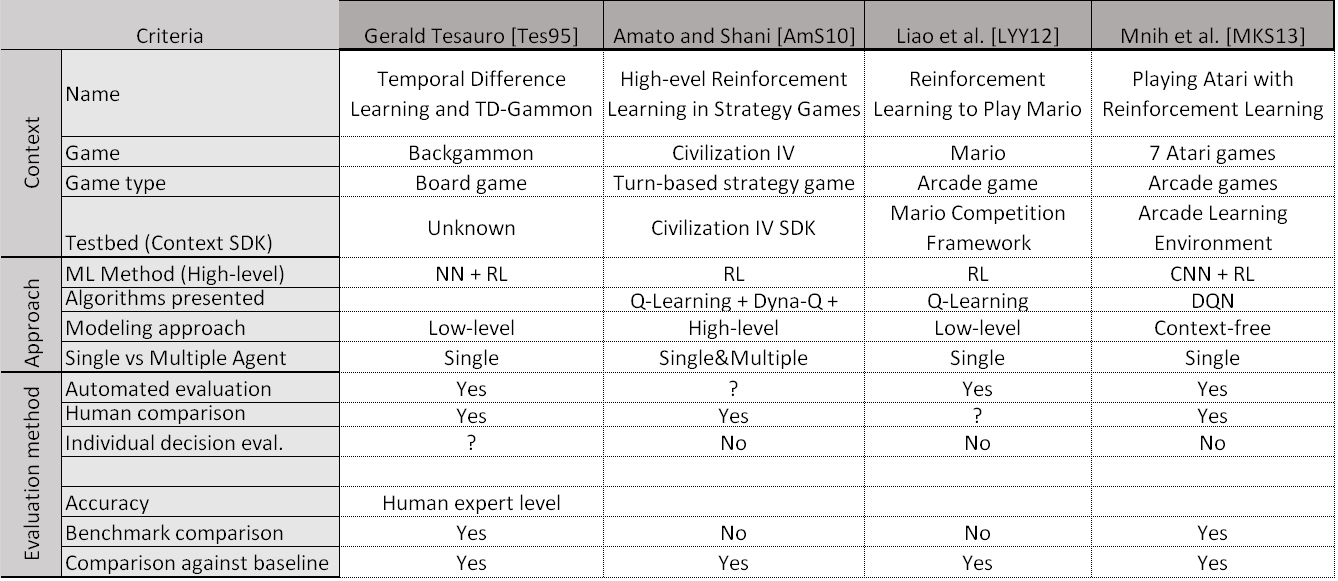
\includegraphics[width=1.1\textwidth]{img/comparison.png}
 		\caption{The comparison matrix presents the differences among four reviewed reinforcement learning articles in the gaming context based on the criteria.}
 		\label{table:comparison}
 	\end{center}
 \end{table}


\section{Conclusion}
Reinforcement learning has received recent attention in the last couple of years due to the breakthrough success in the gaming context. Games play the role of the robust playground for the research by providing several advantages. Providing a controlled environment and contributing to the future studies as a test-bed software, perhaps the most important ones. However, we have presented several challenges in this context as well -- implementation perspective, abstraction approaches, evaluation methods, and further difficulties in terms of algorithms. To get more intuition behind the topic, we reviewed four different reinforcement learning systems in the gaming context.

In summary, the first paper presented an agent to play Super Mario Bros using $\varepsilon$\textit{-greedy} Q-learning, a typical reinforcement learning algorithm. The agent achieved a fast convergence and is able to finish the game about 90\% of the time. Second article demonstrated high-level reinforcement learning approach in a turn-based strategy game called Civilization IV. The system exploits the built-in AI of the game to handle low-level actions and switches between high-level strategies(leader traits in the game provides this high-level strategies) to improve the level of play. The article compared three different reinforcement learning approaches, but Dyna-Q method reached the top result against built-in AI. Third article was a first successful approach to use neural network and reinforcement learning together that achieved grandmaster level of play in backgammon game. However, later it is proved that the main factor to reach this level of play was due to training scheme and the dynamics and stochastic environment of the backgammon game. The final paper introduced a new method, where the system does not require game specific information, but only raw images. This context-free approach is realized using convolutional neural network and Q-learning with experience replay mechanism. After many training stages in Arcade Learning Environment, the agent is able to outperform every existing reinforcement learning approaches and surpassed human experts in 3 out of 7 Atari games. 

We believe that the current trend will be towards the context-free approach, because of its success and applicability. So that the possible future work could be to improve this approach further by extending it to "pure context-free" approach. That is, training the agent with no game specific information and outside of the intended game. In fact, the latter part has been already achieved in neural networks \cite{sukhbaatar2015mazebase}. It would be interesting to investigate the similar approach whether can be applied into convolutional neural networks. 
\newpage
\nocite{*}
\bibliographystyle{tktl}
\bibliography{lahteet}

\lastpage

\appendices

\pagestyle{empty}



\end{document}


